% !TeX program = xelatex
\documentclass[a4paper,10pt]{article}

% ============================================================================
% ១. កញ្ចប់បណ្ណាល័យ និងការកំណត់ទំព័រ (Packages & Page Setup — តាមគំរូ ls_plan.tex)
% ============================================================================
\usepackage[a4paper, left=0.95cm, right=0.95cm, top=0.85cm, bottom=0.92cm, footskip=0.52cm]{geometry}
\usepackage{amsmath}
\usepackage{unicode-math}
\usepackage{fontspec}
\usepackage{longtable, array, multirow, colortbl}
\usepackage[table]{xcolor}
\usepackage{enumitem}
\usepackage{pifont}
\usepackage{fancyhdr}
\usepackage{tikz}
\usetikzlibrary{calc, arrows.meta, decorations.pathreplacing, patterns, positioning, babel}

\makeatletter
\let\@expl@@@mark@update@singlecol@structures@@\relax
\makeatother

% --- ប្រព័ន្ធស្វែងរកទីតាំងពុម្ពអក្សរស្វ័យប្រវត្តិ (Windows Local + Cloud Repo fonts/) ---
\providecommand{\NGSFindFonts}{%
  \IfFileExists{C:/Windows/Fonts/cambria.ttc}{%
    \def\NGSSysPath{C:/Windows/Fonts/}%
    \def\NGSUserPath{C:/Users/KIT/AppData/Local/Microsoft/Windows/Fonts/}%
  }{%
    \IfFileExists{./fonts/KhmerOSsiemreap.ttf}{\def\NGSSysPath{./fonts/}\def\NGSUserPath{./fonts/}}{%
    \IfFileExists{../fonts/KhmerOSsiemreap.ttf}{\def\NGSSysPath{../fonts/}\def\NGSUserPath{../fonts/}}{%
    \IfFileExists{../../fonts/KhmerOSsiemreap.ttf}{\def\NGSSysPath{../../fonts/}\def\NGSUserPath{../../fonts/}}{%
    \IfFileExists{../../../fonts/KhmerOSsiemreap.ttf}{\def\NGSSysPath{../../../fonts/}\def\NGSUserPath{../../../fonts/}}{%
    \IfFileExists{../../../../fonts/KhmerOSsiemreap.ttf}{\def\NGSSysPath{../../../../fonts/}\def\NGSUserPath{../../../../fonts/}}{%
    \IfFileExists{../../../../../fonts/KhmerOSsiemreap.ttf}{\def\NGSSysPath{../../../../../fonts/}\def\NGSUserPath{../../../../../fonts/}}{%
    \IfFileExists{../../../../../../fonts/KhmerOSsiemreap.ttf}{\def\NGSSysPath{../../../../../../fonts/}\def\NGSUserPath{../../../../../../fonts/}}{%
      \def\NGSSysPath{../../../../../../../fonts/}\def\NGSUserPath{../../../../../../../fonts/}%
    }}}}}}}%
  }%
}
\NGSFindFonts

% ============================================================================
% ២. កំណត់ពុម្ពអក្សរ (Fonts — តាមគំរូ ls_plan.tex)
% ============================================================================
\setmathfont[Path={\NGSSysPath}, FontIndex=1, Scale=1.02]{cambria.ttc}
\defaultfontfeatures{Ligatures=TeX}

\setmainfont[
  Path={\NGSUserPath},
  Extension=.ttf,
  Script=Khmer,
  BoldFont={KhmerOSsiemreap},
  BoldFeatures={FakeBold=1.8},
  ItalicFont={KhmerOSsiemreap},
  ItalicFeatures={FakeSlant=0.25},
  BoldItalicFont={KhmerOSsiemreap},
  BoldItalicFeatures={FakeBold=1.8, FakeSlant=0.25}
]{KhmerOSsiemreap}

\newfontfamily\muol[Path={\NGSUserPath}, Extension=.ttf, Script=Khmer]{KhmerOSmuollight}
\newfontfamily\Tacteing[Path={\NGSUserPath}, Extension=.TTF]{TACTENG}
\newfontfamily\TimesEn[Path={\NGSSysPath}, Extension=.ttf, BoldFont={timesbd}, ItalicFont={timesi}, BoldItalicFont={timesbi}]{times}
\newfontfamily\CalibriFont[Path={\NGSSysPath}, Extension=.ttf]{calibri}
\newfontfamily\CourierCirc[Path={\NGSSysPath}, Extension=.ttf]{cour}

\XeTeXlinebreaklocale "km"
\XeTeXlinebreakskip = 0pt plus 1pt minus 0.1pt

% ============================================================================
% ៣. ពណ៌ និងការតុបតែង (Colors & Styles)
% ============================================================================
\definecolor{stepbg}{HTML}{D9D9D9}
\definecolor{headgray}{HTML}{E6E6E6}
\definecolor{emphred}{HTML}{C00000}

\pagestyle{fancy}
\fancyhf{}
\renewcommand{\headrulewidth}{0pt}
\fancyfoot[R]{\CalibriFont\fontsize{9pt}{11pt}\selectfont\thepage}

\setlength{\parindent}{0pt}
\setlength{\parskip}{0pt}
\setlength{\tabcolsep}{4.5pt}
\setlength{\LTpre}{2pt}
\setlength{\LTpost}{2pt}

\newcolumntype{L}[1]{>{\raggedright\arraybackslash}p{#1}}
\newcolumntype{C}[1]{>{\centering\arraybackslash}p{#1}}

% ============================================================================
% ៤. ពាក្យបញ្ជាជំនួយ (Helper Macros)
% ============================================================================
\newcommand{\en}[1]{{\TimesEn #1}}
\newcommand{\enbf}[1]{{\TimesEn\bfseries #1}}
\newcommand{\khmflourish}{{\Tacteing\fontsize{15pt}{15pt}\selectfont 3}}
\newcommand{\wcirc}{{\CourierCirc\fontsize{9.5pt}{11pt}\selectfont o}}
\newcommand{\ditem}{{\fontsize{7.5pt}{10pt}\selectfont\ding{117}}\ }
\newcommand{\fiveE}[1]{\textcolor{emphred}{\CalibriFont\bfseries #1}}
\newcommand{\redsub}[1]{\textcolor{emphred}{#1}}
\newcommand{\timenote}[1]{\textcolor{emphred}{\textit{#1}}}
\newcommand{\stepheader}[1]{\multicolumn{3}{|c|}{\cellcolor{stepbg}\muol #1} \\ \hline}
\newcommand{\cfig}[1]{{\centering\vspace{3pt}#1\vspace{3pt}\par}}
\newcommand{\cnum}[1]{\mbox{\fontsize{10.5pt}{12pt}\selectfont\ding{\numexpr181+#1\relax}}}
\newcommand{\unit}[1]{\,\text{\en{#1}}}
\newcommand{\riel}{\,\text{៛}}
\newcommand{\graybox}[1]{\colorbox{headgray}{\strut #1}}

% ============================================================================
% ៥. រូបភាព TikZ ស-ខ្មៅ សម្រាប់បង្រៀនលើក្ដារខៀន និងសន្លឹកកិច្ចការ (B&W Diagrams)
% ============================================================================

% ១. E1 Engage: អន្ទាក់គូបនៃទ្វេធា (x + 1)^3 = x^3 + 1 vs x^3 + 3x^2 + 3x + 1
\newcommand{\figEngageALGFiveSix}{%
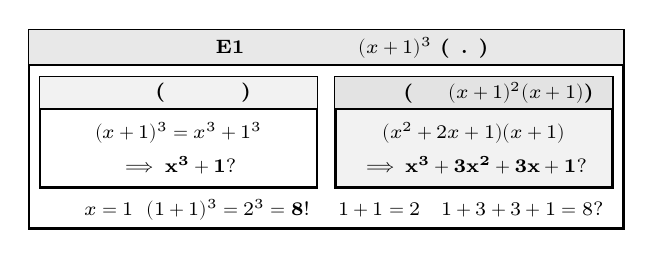
\begin{tikzpicture}[x=1cm, y=1cm, every node/.style={font=\scriptsize, text=black}]
  \draw[black, line width=0.9pt] (0,0) rectangle (7.55,2.52);
  \fill[gray!18] (0,2.08) rectangle (7.55,2.52);
  \draw[black, line width=0.6pt] (0,2.08) -- (7.55,2.08);
  \node at (3.775,2.30) {\textbf{បេសកកម្ម \en{E1}៖ ពន្លាតគូបនៃទ្វេធា $(x + 1)^3$ (ទំ.៦៦)}};

  % Student A
  \draw[black, line width=0.8pt] (0.14,0.52) rectangle (3.66,1.92);
  \fill[gray!10] (0.14,1.52) rectangle (3.66,1.92);
  \draw[black, line width=0.5pt] (0.14,1.52) -- (3.66,1.52);
  \node at (1.90,1.72) {\textbf{សិស្ស ក (លើកគូបដាច់គ្នា)}};
  \node at (1.90,1.22) {$(x+1)^3 = x^3 + 1^3$};
  \node at (1.90,0.80) {$\implies \mathbf{x^3 + 1}$?};

  % Student B
  \draw[black, line width=0.95pt, fill=gray!10] (3.89,0.52) rectangle (7.41,1.92);
  \fill[gray!22] (3.89,1.52) rectangle (7.41,1.92);
  \draw[black, line width=0.55pt] (3.89,1.52) -- (7.41,1.52);
  \node at (5.65,1.72) {\textbf{សិស្ស ខ (បំបែក $(x+1)^2(x+1)$)}};
  \node at (5.65,1.22) {$(x^2+2x+1)(x+1)$};
  \node at (5.65,0.80) {$\implies \mathbf{x^3 + 3x^2 + 3x + 1}$?};

  \node at (3.775,0.24) {\textbf{តេស្ត $x = 1$៖} $(1+1)^3 = 2^3 = \mathbf{8}$! តើ $1+1=2$ ឬ $1+3+3+1=8$?};
\end{tikzpicture}}

% ២. E2 Explore: ត្រីកោណប៉ាស្កាល់ (ទំ.៦៨) និងស៊ីសងតួកណ្ដាល a^3 +- b^3 (ទំ.៦៧)
\newcommand{\figExploreALGFiveSix}{%
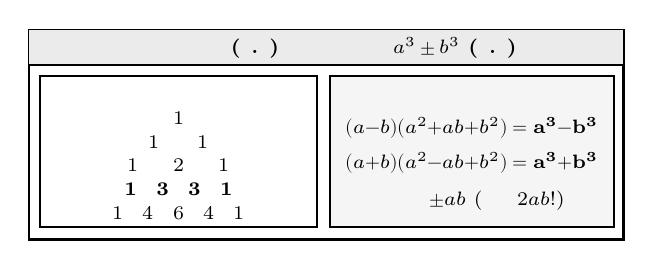
\begin{tikzpicture}[x=1cm, y=1cm, every node/.style={font=\scriptsize, text=black}]
  \draw[black, line width=0.9pt] (0,0) rectangle (7.55,2.66);
  \fill[gray!16] (0,2.22) rectangle (7.55,2.66);
  \draw[black, line width=0.6pt] (0,2.22) -- (7.55,2.22);
  \node at (3.775,2.44) {\textbf{ត្រីកោណប៉ាស្កាល់ (ទំ.៦៨) និងការស៊ីសងតួក្នុង $a^3 \pm b^3$ (ទំ.៦៧)}};

  % Left: Pascal's Triangle n=0..4
  \draw[black, line width=0.8pt] (0.14,0.16) rectangle (3.66,2.08);
  \node at (1.90,1.88) {\textbf{ត្រីកោណប៉ាស្កាល់}};
  \node at (1.90,1.54) {$1$};
  \node at (1.90,1.24) {$1 \qquad 1$};
  \node at (1.90,0.94) {$1 \quad\ \ 2 \quad\ \ 1$};
  \node at (1.90,0.64) {$\mathbf{1 \quad 3 \quad 3 \quad 1}$};
  \node at (1.90,0.34) {$1 \quad 4 \quad 6 \quad 4 \quad 1$};

  % Right: a^3 - b^3 and a^3 + b^3
  \draw[black, line width=0.8pt, fill=gray!8] (3.82,0.16) rectangle (7.43,2.08);
  \node at (5.625,1.86) {\textbf{ផលដកគូប និងផលបូកគូប}};
  \node at (5.625,1.42) {$(a{-}b)(a^2{+}ab{+}b^2) = \mathbf{a^3{-}b^3}$};
  \node at (5.625,0.98) {$(a{+}b)(a^2{-}ab{+}b^2) = \mathbf{a^3{+}b^3}$};
  \node at (5.625,0.50) {ត្រីធាគឺ $\pm ab$ (គ្មាន $2ab$!)};
\end{tikzpicture}}

% ៣. E3 Explain: សង្ខេបរូបមន្តគូបទាំង ៤ (4)--(7) (ទំ.៦៦--៦៨)
\newcommand{\figRuleALGFiveSix}{%
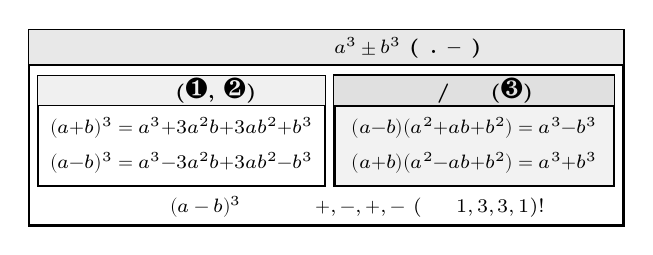
\begin{tikzpicture}[x=1cm, y=1cm, every node/.style={font=\scriptsize, text=black}]
  \draw[black, line width=0.9pt] (0,0) rectangle (7.55,2.48);
  \fill[gray!18] (0,2.04) rectangle (7.55,2.48);
  \draw[black, line width=0.6pt] (0,2.04) -- (7.55,2.04);
  \node at (3.775,2.26) {\textbf{រូបមន្តសង្ខេបគូបនៃទ្វេធា និង $a^3 \pm b^3$ (ទំ.៦៦--៦៨)}};

  % Left: (a+-b)^3
  \draw[black, line width=0.8pt] (0.12,0.50) rectangle (3.76,1.90);
  \fill[gray!12] (0.12,1.52) rectangle (3.76,1.90);
  \draw[black, line width=0.55pt] (0.12,1.52) -- (3.76,1.52);
  \node at (1.94,1.71) {\textbf{គូបនៃទ្វេធា (\cnum{1}, \cnum{2})}};
  \node at (1.94,1.24) {$(a{+}b)^3 = a^3{+}3a^2b{+}3ab^2{+}b^3$};
  \node at (1.94,0.80) {$(a{-}b)^3 = a^3{-}3a^2b{+}3ab^2{-}b^3$};

  % Right: a^3 +- b^3
  \draw[black, line width=0.95pt, fill=gray!10] (3.88,0.50) rectangle (7.43,1.90);
  \fill[gray!24] (3.88,1.52) rectangle (7.43,1.90);
  \draw[black, line width=0.6pt] (3.88,1.52) -- (7.43,1.52);
  \node at (5.655,1.71) {\textbf{ផលដក/បូកគូប (\cnum{3})}};
  \node at (5.655,1.24) {$(a{-}b)(a^2{+}ab{+}b^2) = a^3{-}b^3$};
  \node at (5.655,0.80) {$(a{+}b)(a^2{-}ab{+}b^2) = a^3{+}b^3$};

  \node at (3.775,0.24) {\textbf{លំនាំសញ្ញា $(a-b)^3$៖} ឆ្លាស់គ្នា $+, -, +, -$ (មេគុណ $1, 3, 3, 1$)!};
\end{tikzpicture}}

% ៤. E4 Elaborate: ពន្លាតគូបមានមេគុណ និង (x+1)^4 (ទំ.៦៦--៦៨)
\newcommand{\figElaborateALGFiveSix}{%
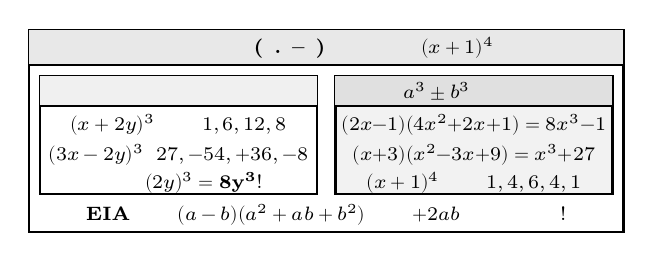
\begin{tikzpicture}[x=1cm, y=1cm, every node/.style={font=\scriptsize, text=black}]
  \draw[black, line width=0.9pt] (0,0) rectangle (7.55,2.56);
  \fill[gray!18] (0,2.12) rectangle (7.55,2.56);
  \draw[black, line width=0.6pt] (0,2.12) -- (7.55,2.12);
  \node at (3.775,2.34) {\textbf{លំហាត់គំរូពង្រីក (ទំ.៦៦--៦៨)៖ គូបទ្វេធា និង $(x+1)^4$}};

  % Left
  \draw[black, line width=0.8pt] (0.14,0.48) rectangle (3.66,1.98);
  \fill[gray!12] (0.14,1.60) rectangle (3.66,1.98);
  \draw[black, line width=0.55pt] (0.14,1.60) -- (3.66,1.60);
  \node at (1.90,1.79) {\textbf{ពន្លាតគូបមានមេគុណ}};
  \node at (1.90,1.36) {$(x+2y)^3$៖ មេគុណ $1, 6, 12, 8$};
  \node at (1.90,0.98) {$(3x-2y)^3$៖ $27, -54, +36, -8$};
  \node at (1.90,0.62) {ប្រយ័ត្ន $(2y)^3 = \mathbf{8y^3}$!};

  % Right
  \draw[black, line width=0.95pt, fill=gray!10] (3.89,0.48) rectangle (7.41,1.98);
  \fill[gray!24] (3.89,1.60) rectangle (7.41,1.98);
  \draw[black, line width=0.6pt] (3.89,1.60) -- (7.41,1.60);
  \node at (5.65,1.79) {\textbf{$a^3\pm b^3$ និងប៉ាស្កាល់}};
  \node at (5.65,1.36) {$(2x{-}1)(4x^2{+}2x{+}1) = 8x^3{-}1$};
  \node at (5.65,0.98) {$(x{+}3)(x^2{-}3x{+}9) = x^3{+}27$};
  \node at (5.65,0.62) {$(x+1)^4$៖ មេគុណ $1,4,6,4,1$};

  \node at (3.775,0.22) {\textbf{\en{EIA}៖} ក្នុង $(a-b)(a^2+ab+b^2)$ បើដាក់ $+2ab$ នឹងស៊ីសងមិនដាច់ទេ!};
\end{tikzpicture}}

% ៥. E5 Evaluate: ជម្រើសវិនិច្ឆ័យ A-D ពន្លាត (x - 2)^3
\newcommand{\figExitALGFiveSix}{%
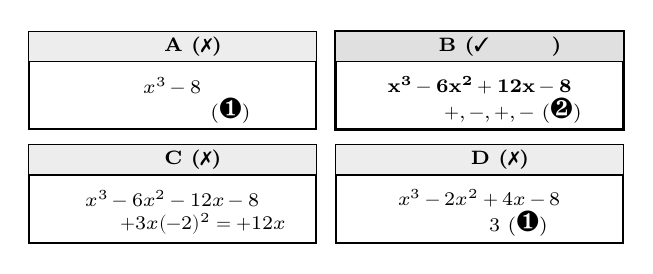
\begin{tikzpicture}[x=1cm, y=1cm, every node/.style={font=\scriptsize, text=black}]
  % Choice A
  \draw[black, line width=0.8pt] (0,1.44) rectangle (3.65,2.68);
  \fill[gray!14] (0,2.30) rectangle (3.65,2.68);
  \draw[black, line width=0.5pt] (0,2.30) -- (3.65,2.30);
  \node at (1.825,2.49) {\textbf{ជម្រើស \en{A} (\ding{55})}};
  \node at (1.825,2.00) {$x^3 - 8$};
  \node at (1.825,1.68) {ភ្លេចតួកណ្ដាលទាំងពីរ (\cnum{1})};

  % Choice B (Correct)
  \draw[black, line width=1.05pt] (3.90,1.44) rectangle (7.55,2.68);
  \fill[gray!24] (3.90,2.30) rectangle (7.55,2.68);
  \draw[black, line width=0.6pt] (3.90,2.30) -- (7.55,2.30);
  \node at (5.725,2.49) {\textbf{ជម្រើស \en{B} (\ding{51} ត្រឹមត្រូវ)}};
  \node at (5.725,2.00) {$\mathbf{x^3 - 6x^2 + 12x - 8}$};
  \node at (5.725,1.68) {សញ្ញាឆ្លាស់ $+, -, +, -$ (\cnum{2})};

  % Choice C
  \draw[black, line width=0.8pt] (0,0) rectangle (3.65,1.24);
  \fill[gray!14] (0,0.86) rectangle (3.65,1.24);
  \draw[black, line width=0.5pt] (0,0.86) -- (3.65,0.86);
  \node at (1.825,1.05) {\textbf{ជម្រើស \en{C} (\ding{55})}};
  \node at (1.825,0.56) {$x^3 - 6x^2 - 12x - 8$};
  \node at (1.825,0.24) {ខុសសញ្ញាតួ $+3x(-2)^2 = +12x$};

  % Choice D
  \draw[black, line width=0.8pt] (3.90,0) rectangle (7.55,1.24);
  \fill[gray!14] (3.90,0.86) rectangle (7.55,1.24);
  \draw[black, line width=0.5pt] (3.90,0.86) -- (7.55,0.86);
  \node at (5.725,1.05) {\textbf{ជម្រើស \en{D} (\ding{55})}};
  \node at (5.725,0.56) {$x^3 - 2x^2 + 4x - 8$};
  \node at (5.725,0.24) {ភ្លេចគុណមេគុណ $3$ (\cnum{1})};
\end{tikzpicture}}

\begin{document}
\fontsize{10pt}{15.2pt}\selectfont

% ============================================================================
% ក្បាលរដ្ឋបាល (Administrative Header — តាមគំរូ ls_plan.tex)
% ============================================================================
{\centering
  {\muol\fontsize{11pt}{16pt}\selectfont ព្រះរាជាណាចក្រកម្ពុជា\par}
  {\muol\fontsize{11pt}{16pt}\selectfont ជាតិ សាសនា ព្រះមហាក្សត្រ\par}
  \vspace{-3pt}{\khmflourish\par}
}

\vspace{1pt}
{\muol\fontsize{10pt}{15.5pt}\selectfont
មន្ទីរអប់រំ យុវជន និងកីឡា ខេត្តកំពង់ធំ\par
ការិយាល័យអប់រំ យុវជន និងកីឡា ស្រុកកំពង់ស្វាយ\par
អនុវិទ្យាល័យព្រះក្រសាំង\par}

\vspace{2pt}
{\centering{\muol\fontsize{11.5pt}{17pt}\selectfont កិច្ចតែងការបង្រៀន\par}}
\vspace{2pt}

% --- ព័ត៌មានទូទៅ ---
{\hspace*{2.8cm}\renewcommand{\arraystretch}{1.08}
\begin{tabular}{@{}l@{\hspace{0.35cm}}p{2.9cm}@{\hspace{0.15cm}}c@{\hspace{0.25cm}}l@{}}
  - & មុខវិជ្ជា & : & គណិតវិទ្យា ថ្នាក់ទី៨ (ពីជគណិត) \\
  - & ចំណងជើងមេរៀន & : & មេរៀនទី៥៖ កន្សោមពីជគណិត \\
  - & ចំណងជើងរង & : & ៣.២ ពន្លាតគូបនៃទ្វេធា ផលដកនិងផលបូកគូប និងត្រីកោណប៉ាស្កាល់ \\
  - & រយៈពេល & : & ១ ម៉ោងសិក្សា (៥០ នាទី) \\
  - & បង្រៀនដោយ & : & ហុក ប៊ុនថែន \\
  - & កាលបរិច្ឆេទ & : & ថ្ងៃព្រហស្បតិ៍ ទី១០ ខែធ្នូ ឆ្នាំ២០២៦ \\
\end{tabular}\par}

\vspace{2pt}

% --- I. វត្ថុបំណង ---
{\muol\fontsize{10pt}{15.5pt}\selectfont \enbf{I.} វត្ថុបំណង\par}
\vspace{1pt}
{\renewcommand{\arraystretch}{1.10}
\begin{tabular}{@{}p{0.55cm}@{}p{2.35cm}@{\hspace{0.15cm}}c@{\hspace{0.25cm}}p{14.95cm}@{}}
  \hfill\wcirc\hspace{0.2cm} & វិជ្ជាសម្បទា & : & សិស្សប្រាប់រូបមន្តសមភាពសំខាន់ៗគូបទាំង ៤ គឺ $(a+b)^3$, $(a-b)^3$, $a^3-b^3$, $a^3+b^3$ និងរបៀបបង្កើតមេគុណតាមត្រីកោណប៉ាស្កាល់បានត្រឹមត្រូវ (ទំ.៦៦--៦៨) ។ \\
  \hfill\wcirc\hspace{0.2cm} & បំណិនសម្បទា & : & សិស្សពន្លាតគូបនៃទ្វេធា និងផលគុណ $(a\mp b)(a^2\pm ab+b^2)$ លើសន្លឹកកិច្ចការបានត្រឹមត្រូវតាមលំនាំសញ្ញា និងមេគុណ ។ \\
  \hfill\wcirc\hspace{0.2cm} & ចរិយាសម្បទា & : & សិស្សមានទម្លាប់ពិនិត្យលំនាំសញ្ញាឆ្លាស់ $+, -, +, -$ និងមេគុណប្រកបដោយភាពហ្មត់ចត់ និងស្មារតីសហការក្នុងក្រុម ។ \\
\end{tabular}\par}

\vspace{2pt}

% --- II. សម្ភារៈឧបទេស ---
{\muol\fontsize{10pt}{15.5pt}\selectfont \enbf{II.} សម្ភារៈឧបទេស\par}
\vspace{1pt}
\hspace*{0.55cm}$\bullet$\ សៀវភៅសិក្សាគោលថ្នាក់ទី៨ (ទំ.៦៦--៦៨, ៧៣) ក្ដារខៀន ដីស/ហ្វឺត បន្ទាត់ត្រង់ និង\textbf{សន្លឹកកិច្ចការសិស្សបំពេញចន្លោះ ស-ខ្មៅ} (កូដ \en{ALG56} ទំព័រ ១--២ សម្រាប់សិស្ស និងទំព័រ ៣ ប្លង់ក្ដារខៀន/ចម្លើយគ្រូ — គ្មានប្រើ \en{LCD})\par

\vspace{2pt}

% --- III. វិធីសាស្រ្តបង្រៀន ---
{\muol\fontsize{10pt}{15.5pt}\selectfont \enbf{III.} វិធីសាស្រ្តបង្រៀន\par}
\vspace{1pt}
{\renewcommand{\arraystretch}{1.08}
\begin{tabular}{@{}p{0.55cm}@{}p{2.35cm}@{\hspace{0.15cm}}c@{\hspace{0.25cm}}p{14.95cm}@{}}
  \hfill$\bullet$\hspace{0.2cm} & គោលវិធី & : & សិស្សមជ្ឈមណ្ឌល (សន្លឹកកិច្ចការបំពេញចន្លោះជាគោល + ការពិភាក្សាជាក្រុមតូច ៣ នាក់) \\
  \hfill$\bullet$\hspace{0.2cm} & យុទ្ធវិធីបង្រៀន & : & គំរូស្ថាបនានិយម \en{5Es} រួមបញ្ចូល \textbf{ការស្វែងរកលំនាំមេគុណតាមត្រីកោណប៉ាស្កាល់} និង \textbf{ការសង្កេតការស៊ីសងតួកណ្ដាលក្នុង $a^3\pm b^3$} \\
\end{tabular}\par}

\vspace{2pt}

% --- IV. ដំណើរការបង្រៀន ---
{\muol\fontsize{10pt}{15.5pt}\selectfont \enbf{IV.} ដំណើរការបង្រៀន\par}

{\renewcommand{\arraystretch}{1.15}
\begin{longtable}{|L{5.50cm}|L{7.90cm}|L{4.80cm}|}
\hline
\multicolumn{1}{|c|}{\cellcolor{headgray}\muol សកម្មភាពគ្រូ} &
\multicolumn{1}{c|}{\cellcolor{headgray}\muol ខ្លឹមសារមេរៀន} &
\multicolumn{1}{c|}{\cellcolor{headgray}\muol សកម្មភាពសិស្ស} \\
\hline
\endfirsthead

\hline
\multicolumn{1}{|c|}{\cellcolor{headgray}\muol សកម្មភាពគ្រូ} &
\multicolumn{1}{c|}{\cellcolor{headgray}\muol ខ្លឹមសារមេរៀន} &
\multicolumn{1}{c|}{\cellcolor{headgray}\muol សកម្មភាពសិស្ស} \\
\hline
\endhead

% ==================== ជំហានទី១ (2min) ====================
\stepheader{ជំហានទី១ \enbf{(}រដ្ឋបាលថ្នាក់\enbf{)}}
$\bullet$ ពិនិត្យវត្តមាន អនាម័យ និងសណ្ដាប់ធ្នាប់ថ្នាក់រៀន \par
$\bullet$ រៀបចំក្រុមតូច ៣ នាក់ និងចែក\textbf{សន្លឹកកិច្ចការសិស្ស (\en{ALG56} ទំព័រ ១–២)}
&
$\bullet$ រដ្ឋបាលថ្នាក់ អនាម័យ និងវិន័យសិក្សា \par
$\bullet$ ចែកសន្លឹកកិច្ចការម្នាក់ ១ សន្លឹក សម្រាប់បំពេញតាមដំណាក់កាល \en{E1--E5}
&
$\circ$ ប្រធានថ្នាក់រាយការណ៍វត្តមានសិស្ស \par
$\circ$ ទទួលសន្លឹកកិច្ចការ សរសេរឈ្មោះ និងអង្គុយតាមក្រុម ៣ នាក់ \\
\hline

% ==================== ជំហានទី២ (9min: កំណែ <=3m + រំលឹក 3m + E1 3m) ====================
\stepheader{ជំហានទី២ \enbf{(}កិច្ចការផ្ទះ \enbf{+} ទំនាក់ទំនងមេរៀនថ្មី\enbf{)}}
\ditem \textbf{កំណែកិច្ចការផ្ទះ ($\le\text{\enbf{3\,min}}$)} \par
$\bullet$ ហៅសិស្ស ២ នាក់ឡើងកែលំហាត់ទំ.៦៤–៦៥ និងទំ.៧៣ \#8 ក, \#9 លើក្ដារខៀន
&
{\centering\redsub{កំណែកិច្ចការផ្ទះ (ទំ.៦៤–៦៥ និង ទំ.៧៣ \#8, \#9)}\par}
$\bullet$ \textbf{ទំ.៦៤–៦៥៖} $(3a-2b)^2 = \mathbf{9a^2-12ab+4b^2}$; \ $(\tfrac{1}{5}t-u)(\tfrac{1}{5}t+u) = \mathbf{\tfrac{1}{25}t^2-u^2}$ \par
$\bullet$ \textbf{\#8 ក៖} $\mathbf{1-x^4}$; \quad \textbf{\#9៖} $54\times 66 = \mathbf{3\,564}$; \ $102^2-101^2 = \mathbf{203}$
&
$\circ$ ផ្ទៀងចម្លើយ និងកែតម្រូវចូលសៀវភៅកិច្ចការផ្ទះ \\[3pt]

\ditem \textbf{រំលឹកមេរៀនទាក់ទង (\enbf{3min})} \par
$\bullet$ សួរ៖ «តើ $(a+b)^2$ និង $(a-b)^2$ ស្មើអ្វី? ចុះ $(-2y)^2$ និង $(-2y)^3$ ស្មើប៉ុន្មាន?»
&
{\centering\redsub{រំលឹកការេនៃទ្វេធា និងស្វ័យគុណគូ/សេសនៃចំនួនអវិជ្ជមាន}\par}
$\bullet$ $(a\pm b)^2 = a^2 \pm 2ab + b^2$ \par
$\bullet$ $(-2y)^2 = \mathbf{+4y^2}$ (គូ $\to +$) \quad ឯ \quad $(-2y)^3 = \mathbf{-8y^3}$ (សេស $\to -$)
&
$\circ$ ឆ្លើយ៖ «$a^2\pm 2ab+b^2$; $+4y^2$; និង $-8y^3$!» \\[3pt]

\fiveE{E1 - Engage (3min)} \timenote{(កុំទាន់ផ្ដល់ចម្លើយ)} \par
\ditem \textbf{បេសកកម្មអន្ទាក់គូបនៃទ្វេធា (សន្លឹកកិច្ចការ \en{E1})} \par
$\bullet$ ឱ្យសិស្សអានប្រអប់ \en{E1} ហើយតេស្តដោយជំនួស $x = 1$ ដើម្បីជ្រើសរើសរវាង\textbf{សិស្ស ក} និង\textbf{សិស្ស ខ}
&
\redsub{បេសកកម្ម \en{E1}៖ ពន្លាតគូបនៃទ្វេធា $(x + 1)^3$ (ទំ.៦៦)} \par
$\bullet$ \textbf{សិស្ស ក} លើកគូបដាច់គ្នា បាន $x^3 + 1^3 = x^3 + 1$! \par
$\bullet$ \textbf{សិស្ស ខ} គុណ $(x+1)^2(x+1)$ បាន $x^3 + 3x^2 + 3x + 1$! តើអ្នកណាត្រូវ?
&
$\circ$ ជំនួស $x=1$ ពិភាក្សាជាគូ និងគូស \ding{51} ក្នុងប្រអប់ \en{E1} \\[3pt]

&
\cfig{\figEngageALGFiveSix}
& \\
\hline

% ==================== ជំហានទី៣ (17min: E2 11m + E3 6m) ====================
\stepheader{ជំហានទី៣ \enbf{(}ខ្លឹមសារមេរៀនថ្មី\enbf{)}}
\fiveE{E2 - Explore (11min)} \par
$\bullet$ សរសេរចំណងជើងរង \textbf{៣.២ ពន្លាតគូបនៃទ្វេធា និងត្រីកោណប៉ាស្កាល់} លើក្ដារខៀន \par
\ditem \textbf{សកម្មភាព ១៖ គូបនៃផលបូក និងគូបនៃផលដក (ទំ.៦៦–៦៧, \enbf{6min}, \en{E2-A})} \par
$\bullet$ ឱ្យសិស្សពន្លាត $(a+b)^2(a+b)$ និង $(a-b)(a-b)^2$ លើ \en{E2-A}
&
៣.២ ពន្លាតគូបនៃទ្វេធា (ទំ.៦៦–៦៧) \par
$\bullet$ \textbf{គូបនៃផលបូក (4)៖} $(a+b)^3 = (a^2+2ab+b^2)(a+b) = \mathbf{a^3 + 3a^2b + 3ab^2 + b^3}$ (គំរូ៖ $(x+1)^3 = x^3+3x^2+3x+1$) \par
$\bullet$ \textbf{គូបនៃផលដក (5)៖} $(a-b)^3 = (a-b)(a^2-2ab+b^2) = \mathbf{a^3 - 3a^2b + 3ab^2 - b^3}$ (គំរូ៖ $(x-1)^3 = x^3-3x^2+3x-1$)
&
$\circ$ គុណពន្លាត បង្រួមតួដូចគ្នា និងសង្កេតមេគុណ $1,3,3,1$ លើ \en{E2-A} \\[3pt]

\ditem \textbf{សកម្មភាព ២៖ $a^3\mp b^3$ និងត្រីកោណប៉ាស្កាល់ (ទំ.៦៧–៦៨, \enbf{5min}, \en{E2-B})} \par
$\bullet$ ឱ្យសិស្សពន្លាត $(a\mp b)(a^2\pm ab+b^2)$ និងបំពេញត្រីកោណប៉ាស្កាល់លើ \en{E2-B}
&
ផលដកគូប ផលបូកគូប និងត្រីកោណប៉ាស្កាល់ (ទំ.៦៧–៦៨) \par
$\bullet$ \textbf{រូបមន្ត (6) និង (7)៖} $(a-b)(a^2+ab+b^2) = \mathbf{a^3 - b^3}$; \quad $(a+b)(a^2-ab+b^2) = \mathbf{a^3 + b^3}$ \par
$\bullet$ \textbf{ត្រីកោណប៉ាស្កាល់ (ទំ.៦៨)៖} ជួរទី៣ គឺ $\mathbf{1, 3, 3, 1}$; ជួរទី៤ គឺ $\mathbf{1, 4, 6, 4, 1}$; ជួរទី៥ គឺ $\mathbf{1, 5, 10, 10, 5, 1}$
&
$\circ$ សង្កេតការស៊ីសងតួកណ្ដាល និងបំពេញជួរត្រីកោណប៉ាស្កាល់លើ \en{E2-B} \\[3pt]

&
\cfig{\figExploreALGFiveSix}
& \\[3pt]

% --- E3 Explain (6min) ---
\fiveE{E3 - Explain (6min)} \par
$\bullet$ ដឹកនាំសិស្សសង្ខេបរូបមន្តសមភាពសំខាន់ៗទី (4), (5), (6) និង (7) (ទំ.៦៦–៦៨)
&
$\bullet$ \textbf{រូបមន្តសង្ខេបគូបទាំង ៤ (ទំ.៦៦–៦៨)៖} \par
\hspace*{0.15cm}(4) $(a + b)^3 = \graybox{$a^3 + 3a^2b + 3ab^2 + b^3$}$ \par
\hspace*{0.15cm}(5) $(a - b)^3 = \graybox{$a^3 - 3a^2b + 3ab^2 - b^3$}$ \par
\hspace*{0.15cm}(6) $(a-b)(a^2+ab+b^2) = \mathbf{a^3-b^3}$; \quad (7) $(a+b)(a^2-ab+b^2) = \mathbf{a^3+b^3}$
&
$\circ$ បំពេញប្រអប់រូបមន្តសង្ខេបទាំង ៤ លើ \en{E3} \\[3pt]

$\bullet$ ភ្ជាប់\textbf{ធនាគារហេតុផល \cnum{1}--\cnum{4}} លើក្ដារខៀន និងសន្លឹកកិច្ចការ
&
\textbf{ធនាគារហេតុផល (\en{Warrant Bank})៖} \par
\cnum{1} \textbf{មេគុណ $1, 3, 3, 1$៖} និទស្សន្ត $a$ ថយចុះ ($3\to 0$) រីឯនិទស្សន្ត $b$ កើនឡើង ($0\to 3$) \par
\cnum{2} \textbf{សញ្ញាឆ្លាស់ $(a-b)^3$៖} មានសញ្ញាឆ្លាស់ $+, -, +, -$ ព្រោះ $(-b)^2=+b^2$ និង $(-b)^3=-b^3$
&
$\circ$ ផ្ទៀងលេខកូដ \cnum{1}--\cnum{2} លើសន្លឹកកិច្ចការ \\[3pt]

&
\cnum{3} \textbf{ត្រីធាក្នុង $a^3\mp b^3$៖} តួកណ្ដាលគឺ $\pm ab$ (ហាមដាក់ $\pm 2ab$) និងមានសញ្ញាផ្ទុយពីទ្វេធាខាងមុខ
&
$\circ$ ផ្ទៀងលេខកូដ \cnum{3} លើសន្លឹកកិច្ចការ \\[3pt]

&
\cnum{4} \textbf{ត្រីកោណប៉ាស្កាល់៖} មេគុណកណ្ដាលនីមួយៗស្មើផលបូកពីរមេគុណខាងលើជាប់គ្នា
&
$\circ$ ផ្ទៀងលេខកូដ \cnum{4} លើសន្លឹកកិច្ចការ \\[3pt]

&
\cfig{\figRuleALGFiveSix}
& \\
\hline

% ==================== ជំហានទី៤ (20min: E4 10m + E5 10m) ====================
\stepheader{ជំហានទី៤ \enbf{(}ពង្រីកចំណេះដឹង\enbf{)}}
\fiveE{E4 - Elaborate (10min)} \par
\ditem \textbf{លំហាត់គំរូពង្រីក៖ ប្រតិបត្តិទំ.៦៦–៦៨ និងត្រីកោណប៉ាស្កាល់} \par
$\bullet$ ឱ្យសិស្សធ្វើលំហាត់ទំ.៦៦–៦៧ និងពន្លាត $(x+1)^4$ លើ \en{E4}
&
{\muol លំហាត់គំរូពង្រីក} \textbf{(ទំ.៦៦–៦៨)៖} \par
$\bullet$ \textbf{១) គូបនៃទ្វេធាមានមេគុណ (ទំ.៦៦–៦៧)៖} \par
\hspace*{0.2cm}-- $(x+2y)^3 = x^3 + 3x^2(2y) + 3x(2y)^2 + (2y)^3 = \graybox{$x^3 + 6x^2y + 12xy^2 + 8y^3$}$ \par
\hspace*{0.2cm}-- $(3x-2y)^3 = \mathbf{27x^3 - 54x^2y + 36xy^2 - 8y^3}$ \par
$\bullet$ \textbf{២) ផលគុណ $a^3\pm b^3$ និងត្រីកោណប៉ាស្កាល់ (ទំ.៦៧–៦៨)៖} \par
\hspace*{0.2cm}-- $(2x-1)(4x^2+2x+1) = (2x)^3 - 1^3 = \mathbf{8x^3 - 1}$; \quad $(x+3)(x^2-3x+9) = \mathbf{x^3 + 27}$ \par
\hspace*{0.2cm}-- ជួរទី៤ នៃត្រីកោណប៉ាស្កាល់៖ $(x+1)^4 = \graybox{$x^4 + 4x^3 + 6x^2 + 4x + 1$}$
&
$\circ$ ពន្លាតគូប ផលគុណ $a^3\pm b^3$ និង $(x+1)^4$ លើ \en{E4} ត្រឹមត្រូវ \\[3pt]

&
\cfig{\figElaborateALGFiveSix}
& \\[3pt]

$\bullet$ សួរសំណួរឆ្លុះបញ្ចាំង \textbf{\en{EIA Looking-Back} (1min)}
&
\textbf{\en{EIA Looking-Back}៖} «តើ $(a-b)(a^2+2ab+b^2)$ ស្មើ $a^3-b^3$ ដែរឬទេ? ហេតុអ្វី?» ($\to$ មិនស្មើទេ! ដើម្បីឱ្យតួកណ្ដាលស៊ីសងដាច់សូន្យ ត្រីធាត្រូវតែជា $a^2+ab+b^2$ គ្មានមេគុណ $2$!)
&
$\circ$ ពន្យល់ថាក្នុង $a^3-b^3$ តួកណ្ដាលនៃត្រីធាគឺ $+ab$ (\cnum{3}) \\[3pt]

% --- E5 Evaluate (10min) ---
\fiveE{E5 - Evaluate (10min)} \par
\ditem \textbf{ប្រតិបត្តិជាក្រុមតូច ៣ នាក់ (4min, សន្លឹកកិច្ចការ \en{E5})} \par
$\bullet$ ឱ្យសិស្សដោះស្រាយប្រតិបត្តិទំ.៦៦ (ខ) និងទំ.៦៧ (ខ, គ)
&
{\muol លំហាត់ប្រតិបត្តិ} \textbf{(ទំ.៦៦–៦៧)៖} \par
$\bullet$ \textbf{១) ទំ.៦៦ (ខ) និង ទំ.៦៧ (ខ)៖} $(x+3y)^3 = \mathbf{x^3+9x^2y+27xy^2+27y^3}$; \ $(2x-y)^3 = \mathbf{8x^3-12x^2y+6xy^2-y^3}$ \par
$\bullet$ \textbf{២) ទំ.៦៧ ខាងក្រោម (គ)៖} $(2x+1)(4x^2-2x+1) = (2x)^3 + 1^3 = \mathbf{8x^3 + 1}$
&
$\circ$ គណនាជាក្រុមឃើញគូបទាំងពីរ និង $8x^3+1$ ត្រឹមត្រូវ \\[3pt]

$\bullet$ ឱ្យក្រុមសិស្សផ្ទៀងផ្ទាត់និង\textbf{បិទបេសកកម្ម \en{E1} (2min)}
&
$\bullet$ \textbf{បិទបេសកកម្ម \en{E1}៖} សិស្ស ខ ត្រឹមត្រូវ! $(x+1)^3 = \mathbf{x^3+3x^2+3x+1}$ (ពេល $x=1$: $1+3+3+1 = 8 = 2^3$ \ding{51})!
&
$\circ$ បិទបេសកកម្ម \en{E1} ឃើញសិស្ស ខ ត្រឹមត្រូវ \\[3pt]

\ditem \textbf{សំណួរវិនិច្ឆ័យ \en{A--D} និងសំបុត្រចេញ (4min)} \par
$\bullet$ ឱ្យសិស្សគូសរង្វង់ជម្រើសត្រូវលើសន្លឹកកិច្ចការ រួចលើកម្រាមដៃ ១--៤
&
{\centering\textbf{សំណួរវិនិច្ឆ័យ \en{A--D}៖ ពន្លាតគូបនៃទ្វេធា $(x - 2)^3$}\par}
{\centering \enbf{A.}\ $x^3-8$ \quad \enbf{B.}\ $x^3-6x^2+12x-8$ \quad \enbf{C.}\ $x^3-6x^2-12x-8$ \quad \enbf{D.}\ $x^3-2x^2+4x-8$\par}
{\centering\textit{(កត់សម្គាល់៖ ប្រើមេគុណ $1, 3, 3, 1$ និងសញ្ញាឆ្លាស់ $+, -, +, -$)}\par}
&
$\circ$ គណនា និងលើកម្រាមដៃ ២ (\textbf{ជម្រើស \en{B}៖ $x^3-6x^2+12x-8$}) \\[3pt]

&
\cfig{\figExitALGFiveSix}
& \\[3pt]

$\bullet$ បញ្ជាក់ចម្លើយត្រូវ (\textbf{ជម្រើស \en{B}}) និងឱ្យបំពេញ\textbf{សំបុត្រចេញ ៦០ វិនាទី}
&
$\bullet$ \textbf{សំបុត្រចេញ (ទំ.៦៧ ខ)៖} ពន្លាត $(x - 3)(x^2 + 3x + 9) = x^3 - 3^3 = \mathbf{x^3 - 27}$ ។
&
$\circ$ បំពេញសំបុត្រចេញលើសន្លឹកកិច្ចការមុនបញ្ចប់ម៉ោង \\
\hline

% ==================== ជំហានទី៥ (<=2min) ====================
\stepheader{ជំហានទី៥ \enbf{(}កិច្ចការផ្ទះ \enbf{+} បណ្ដាំផ្ញើ\enbf{)}}
\timenote{ចំណាយពេលឱ្យតិចបំផុតកុំឱ្យលើស 2min} \par
$\bullet$ ណែនាំប្រអប់\textbf{កិច្ចការផ្ទះ}លើសន្លឹកកិច្ចការទំព័រ ២ (ទំ.៦៦–៦៧ និងទំ.៧៣ \#10)
&
{\centering{\muol កិច្ចការផ្ទះ} \textbf{(សៀវភៅគោល ទំ.៦៦–៦៧ និង ទំ.៧៣ \#10 គ, ឃ, ង)}\par} \par
$\bullet$ \textbf{១) ប្រតិបត្តិទំ.៦៦ (គ, ឃ) និង ទំ.៦៧ (ឃ)៖} ពន្លាត $(3x+4y)^3, (\tfrac{1}{5}a+b)^3, (\tfrac{1}{5}t-k)^3$ និង $(\sqrt{2}a-3b)(2a^2+3\sqrt{2}ab+9b^2)$ ។ \par
$\bullet$ \textbf{២) លំហាត់ \#10 គ, ឃ, ង (ទំ.៧៣)៖} ពន្លាតនិងបង្រួម $(a-3b)^2+9(a^2-3b)+5$, $-x(4x-3y)+x^2-12xy$ និង $(x-1)^3-(x+2)^3$ ។
&
$\circ$ គូសចំណាំកិច្ចការផ្ទះលើសន្លឹកកិច្ចការ \\[3pt]

$\bullet$ ផ្ដាំផ្ញើឱ្យអានមុនចំណុច ៤.១–៤.២ (ការដាក់ជាផលគុណកត្តាតាមកត្តារួម និងសមភាពសំខាន់ៗ)
&
$\bullet$ \textbf{បណ្ដាំផ្ញើ៖} អានមុន \textbf{៤.១ កត្តារួម និង ៤.២ ប្រើសមភាពសំខាន់ៗ (ទំ.៦៨–៧០)} ។
&
$\circ$ កត់ត្រាបណ្ដាំផ្ញើ ទុកសន្លឹកកិច្ចការក្នុងសៀវភៅ និងជម្រាបលាគ្រូ \\
\hline
\end{longtable}}

\vspace{6pt}
% --- ហត្ថលេខា (កាលបរិច្ឆេទត្រូវគ្នា ១០០% នឹងខាងលើ) ---
{\centering
\hspace*{5.2cm}\begin{minipage}{11.5cm}
  \centering
  ថ្ងៃព្រហស្បតិ៍ ១កើត ខែមិគសិរ ឆ្នាំមមី អដ្ឋស័ក ពុទ្ធសករាជ ២៥៧០\par
  កំពង់ស្វាយ, ថ្ងៃទី១០ ខែធ្នូ ឆ្នាំ២០២៦\par
  \vspace{2pt}
  {\muol គ្រូបង្រៀន\par}
  \vspace{32pt}
  \hfill{\muol ហុក ប៊ុនថែន}\hspace*{1.4cm}
\end{minipage}\par}

\end{document}
